%%%%%%%%%%%%%%%%%%%%%%%%%%%%%%%%%%%%%%%%%%%%%%%%%%%%%%%%%%%%%%%%%%%%%%%%%%%%%%%%
%2345678901234567890123456789012345678901234567890123456789012345678901234567890
%        1         2         3         4         5         6         7         8

\documentclass[letterpaper, 10 pt]{llncs}

\usepackage[utf8]{inputenc}
\usepackage[T1]{fontenc}
\usepackage{minted}
\usepackage{xcolor}
\usepackage{graphicx}



\title{\LARGE \bf
LLVM address sanitizer specific optimalizations
}


\author{P\'eter K\'okai \and
        Attila Kiss}
%
\authorrunning{P. K\'okai et al.}

\institute{Eotrovs Lorand University, \and
\email{kokaipeter@gmail.com, kiss@inf.elte.hu}
}
%


\usepackage[backend=biber]{biblatex}
\addbibresource{ref.bib}
\let\cite\parencite

\begin{document}



\maketitle
\thispagestyle{empty}
\pagestyle{empty}


%%%%%%%%%%%%%%%%%%%%%%%%%%%%%%%%%%%%%%%%%%%%%%%%%%%%%%%%%%%%%%%%%%%%%%%%%%%%%%%%
\begin{abstract}
The address sanitizer since introduced became a very popular memory related error detection, while there are other tools covering almost the same set of detection, the sanitzer by instrumenting the executable binary itself can be inferior in performance. For some application the performance is critical, thus cannot use properly a more traditional like memory detection tools.
The aim is to find possible ways for performance improvement in the sanitizer code instrumentor.


\end{abstract} \hspace{10pt}

\small \textbf{Keywords} LLVM, address sanitizer, asan, store-load instrument reduce

%%%%%%%%%%%%%%%%%%%%%%%%%%%%%%%%%%%%%%%%%%%%%%%%%%%%%%%%%%%%%%%%%%%%%%%%%%%%%%%%


\section{Introduction}


One of the major advantages of ASAN its performance, the avarage slowdown is 1.75 according to this research\cite{serebryany2012addresssanitizer}. The natural performance gain comes from the nature of instrumenting the code in compile time, and not changing in runtime. Moving a lot of computation to the compiler. Additionally in the LLVM sanitizers are implemented as a LLVM IR\cite{llvm-ir} transformation, just like the optimizers in common named called Passes. There are different type of Passes, despite of their types each Pass is executed in a semi-random order. The sanitizer type of Passes (Address, Memory, Thread, Undefined, etc) are executed in the last place, thus instructions that are removed by optimization are ignored without any effort. As well as the different type of Passes are not required to know about the sanitizer specific implementations.

This effectivly also means that the code generated by the sanitizer is not optimized at all. The question could come naturally if there is a need for further optimizing for those code. One of the factor is the actuall code created by the ASAN itself, and its context the rest of the code. At least the focus in this paper going to be on improvement that can be only done with wide range of code.

The following sections are going to rely heavily on knowladge about LLVM\cite{lattner2008llvm} and its intermediate representation of LLVM IR\cite{llvm-ir}. The LLVM/clang was choosen exactly because of its LLVM IR based design opposed to gcc.

\section{Related works}

\subsection{Sanitizers}
The number of sanitizers are keep growing since the address\cite{serebryany2012addresssanitizer}, leak and memory\cite{stepanov2013memorysanitizer} sanitizer were introduced. There are undefiend behavior, thread, data flow and even hardware support exists for example Intel MPX\cite{oleksenko2018intel}. The application of the ASAN also reached multiple kernel implementation such as the linux kernel, in which there are some differences and called KSAN\cite{reshetova2018toward}. The kernel is the prime example where the common tools such as valgrind are impossible to use. By providing a provisioned binary makes it easier.

\subsection{libFuzzer}
The sanitizer mentioned before here were mostly changing the applications only when some type of violation were detected. Only changed the execution path in case of unsafe behavior, and it did not effect the base functionality of the software. The type of sanitizers do not stop there, there is one particular example called fuzzer. The libFuzzer is implemented as a sanitizer in LLVM/clang, and it is possible to combine with other sanitizers such as ASAN. The combination of libFuzzer and different sets of sanitizers could find security issues in no time. Such an example is the openssl heartbleed\cite{alkazimi2016heartbleed}\cite{bohme2017directed}.

\section{Concepts and problems}

Despite gcc also has sanitizer capability, it is more limited\cite{hytonen2018replacing}. Of course likely the concepts could be later applied for gcc. Now it is best to stick to clang here, and explore only that compiler extensation. The next section is going to explain how any sanitizer fits into the compilation stages of clang.

\subsection{LLVM/Passes}

The clang could be divided into multiple subtasks that take part of transforming the source code into a machine binary. The clang itself heavily utilizes LLVM that has optimization, machine code generation support as well. The clang as a front end should only emit the LLVM IR - intermediate format used by LLVM to create an interface between subtasks. This can be seen in the Figure~\ref{fig:llvm-passes}. The important thing to notice here is the middle end - also exists as opt executable - that takes LLVM IR as an input, and produces the same type of output.

The midle end is responsible for most of the transformation in the build system. While the transformation might not even transform anything at all, and generally called Pass. A Pass simply has access to the parsed LLVM IR, and it is free to make any type of transformation, or in some cases a Pass just reports information to the user. Such example is a Pass that reports information about all of the other Passes.

\begin{figure}[H]
\centering
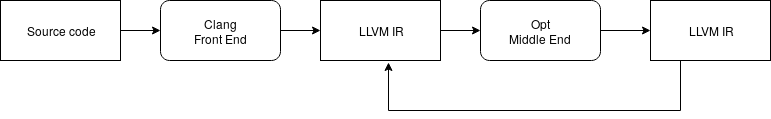
\includegraphics[scale=0.5]{LLVM_Passes.png}
\caption{LLVM/Passes}
\label{fig:llvm-passes}
\end{figure}

Of course as the passes operates on LLVM IR they are independent of the initial language. The passes can be grouped based on the scope they are working: global, function. Also based on the type of transformation they are doing like code optimalization. The optimalizations are also implemented as a Pass. The other important Pass that are already mentioned many time before are the sanitizers. While one sanitizer - like address - does not mean one Pass. It is also possible to define ordering and dependencies between Passes.

\subsection{Sanitizer as Pass}

The address sanitizer is not different, it is implemented as a Pass, in fact it consists of multiple Passes. The address sanitizer must change any code that does store/load instruction and every scope with different lifetime due to function call, or simple block \{\}. By extending the code with the checks in ASAN would make the optimizer jobs really hard or in some cases impossible. Additionally the optimizer might decide to inline function, or remove memory accesses; surely those are not requires any error checking code from any sanitizer. Due to this the sanitizers are ordered in a way that they are executed as the last step. This ensures that the LLVM IR is seen by any sanitizer is as optimizedd as it can be with the current setup.

\subsection{Reoptimize the code}

One could think that even if the LLVM IR the sanitizer starts to work on were initally optimized, currently as the sanitizer is the last one in the execution chain it would be up to the sanitizer to keep it optimized. Which is clearly not the task of any sanitizer, in fact sanitizer does the opposite than keeping the code optimized.

It is easy to see that most likely after the sanitizer the results will not be keep its optimized quality. The simple idea is to use the 


\begin{figure}[H]
\centering
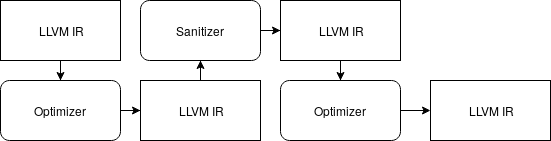
\includegraphics[scale=0.5]{clang-opt-asan-opt.png}
\caption{Optimize + ASAN + Optimize}
\label{fig:opt-asan-opt}
\end{figure}






\begin{minted}{c}
define dso_local void @inc(i32* nocapture %a) #0 {
entry:
  %0 = ptrtoint i32* %a to i64
  call void @__asan_load4(i64 %0)
  %1 = load i32, i32* %a, align 4
  %add = add nsw i32 %1, 1
  %2 = ptrtoint i32* %a to i64
  call void @__asan_store4(i64 %2)
  store i32 %add, i32* %a, align 4
  ret void
}
\end{minted}

\begin{minted}{c}
void d_memset(int *a, int value, int n) {
  for (int i = 0; i < n; ++i) {
    a[i] = value;
  }
}
\end{minted}


\section{Experiments}

\subsection{Naiv approach}

The nice thing about LLVM that it can produce LLVM IR as a result, additionally it can parse it as an input as well. One could simply ask clang to emit LLVM IR, and after that step simple re-execute all of those optimizers on top of it with opt.

By checking the examples above with the afformentioned idea it is possible to identify some change in the code itself. Examint further thoses changes, it is possible to clasify into three different section:
\begin{itemize}
 \item convert function to tail call
 \item change the order from and, add, trunc to trunc, and, add
 \item reverse the branch from true: error handling false: fast path
\end{itemize}

Depending on the decision that sanitizer makes (currently based on the number of instrumention it must take) it could either inject the code itself or just call a function. But either way as just the opt suggested converting those function calls by default tail call is a fine move.

The benefit of working on a 8bit number instead of a 64bit can be doubtful on a 64 bit system, but can be appritiated on a 32 bit system.

The change in the branch is intresting from the branch prediction point of view, the error handling branch performance does not concern us as it also going to terminate the application and only going to happen at most onece. While the fast path should be triggered all the time.

\subsection{Phoronix Test Suite}

The main focus of this work is on the performance of the resulting instrumented binaries, as a result different type of memories like heap or stack will not be investigated. Additionally the build time itself also not in focus, even thoue that is most likely going to increase. One could reason that the build time increase might do not worth the runtime speedup; as the ASAN is generally used during development and runtime, buildtime are both important.

The phoronix test suite\cite{larabel2011phoronix} has a collection of different performance measurement tests. First of all the tests that are closed sourced, or not compiled are not selected for obviouse reasons. Secondly only the test that measure runtime are kept as the goal is to optimize for those.  Further such test that measure the compilation time instead of runtime are not in focus. Filtering out all of those tests provides us with the following tests:

\begin{itemize}
	\item TODO: list here all of the test that were choosen
	\item PTS/sqlite (sql interaction)
	\item PTS/cpp-perf-banch (compiler optimization like loop unroll etc)
	\item 
\end{itemize}


\section{Results}

\subsection{Compare clang and clang with ASAN}

The comparision of clang and clang with ASAN execution is just in order to create a baseline.

\subsection{Compare clang with ASAN and clang with ASAN and opt}

T


\section{Conclusion}

\section{Future works}


\begin{itemize}
	\item Investigate the memory footprint (heap, stack)
	\item Compare the sum of build and compile time (as usually this is used in CI, where both matters)
\end{itemize}


\section*{Acknowledgment}


\printbibliography

\end{document}

